\section{Durchführung}
\label{sec:Durchführung}
In diesem Versuch werden ein Acrylblock und ein Brustmodell mit verschiedenen Ultraschall Scan-Verfahren untersucht. Es genügt nicht die Ultraschallsonde auf das zu untersuchende Material zu halten, da sich dann
zwischen der Sonde und dem Material eine Luftschicht befindet, wodurch die Messung misslingen würde. Um dies zu vermeiden
wird ein Kontaktmittel auf das Material aufgetragen. Für den Acrylblock wird destilliertes Wasser verwendet.
Die Dicke dieser Wasserschicht muss jedoch bei der Auswertung berücksichtigt werden, um systematische Abweichungen zu vermeiden.

\subsection{Vorbereitungsaufgaben}
\label{subsec:VBA}
Wie in \autoref{subsec:Grundlagen} erwähnt, ist die Schallgeschwindigkeit $c$ eine materialabhängige Konstante. Für den folgenden Versuch sind drei 
Schallgeschwindigkeiten relevant. Destilliertes Wasser hat bei $\qty{20}{\celsius}$ eine Schallgeschwindigkeit von $\qty{1483}{\metre\per\second}$,
in Acryl beträgt die Schallgeschwindigkeit $\qty{2730}{\metre\per\second}$ und in Luft (bei $\qty{20}{\celsius}$) $\qty{344}{\metre\per\second}$.
Es werden zwei verschiedene Messsonden verwendet. Eine sendet Ultraschall mit eine Frequenz von $\qty{1}{\mega\hertz}$ und die Andere mit $\qty{2}{\mega\hertz}$. 
Mittels \autoref{eqn:lambda} kann die Wellenlänge und Periodendauer in Acryl bestimmt werden. Dazu wird die zuvor erwähnte Schallgeschwindigkeit
verwendet. Mit einer Frequenz von $\qty{1}{\mega\hertz}$ ergibt sich eine Wellenlänge von $\qty{2.73}{\milli\metre}$ und eine Periodendauer von $\qty{1}{\micro\second}$. 
Bei $\qty{1}{\mega\hertz}$ liegt die Wellenlänge bei $\qty{1.365}{\milli\metre}$ und die Periodendauer bei $\qty{0.5}{\micro\second}$.
\subsection{Versuchsdurchführung}
\label{subsec:Versuchsdurchführung}
Zur Untersuchung mit Ultraschall wird ein Ultraschallechoskop und Ultraschallsonden verschiedener Frequenzen benötigt. Des Weiteren wird ein Acrylblock, welcher
in \autoref{fig:acrylskizze} dargestellt ist, und destilliertes Wasser benötigt. 
Das Ultraschallechoskop wird im Impuls-Echo-Verfahren verwendet. Die Sendefrequenz wird in einem Bereich von $\qty{0}{\decibel}$ bis $\qty{30}{\decibel}$ eingestellt. Die 
Empfängerfrequenz in einem Bereich von $\qty{0}{\decibel}$ bis $\qty{35}{\decibel}$. Das Ultraschallechoskop wird mit einem Computer verbunden, an welchem  
das Programm \textit{A-Scan} die Messwerte verarbeitet. 

\begin{figure}
    \centering
	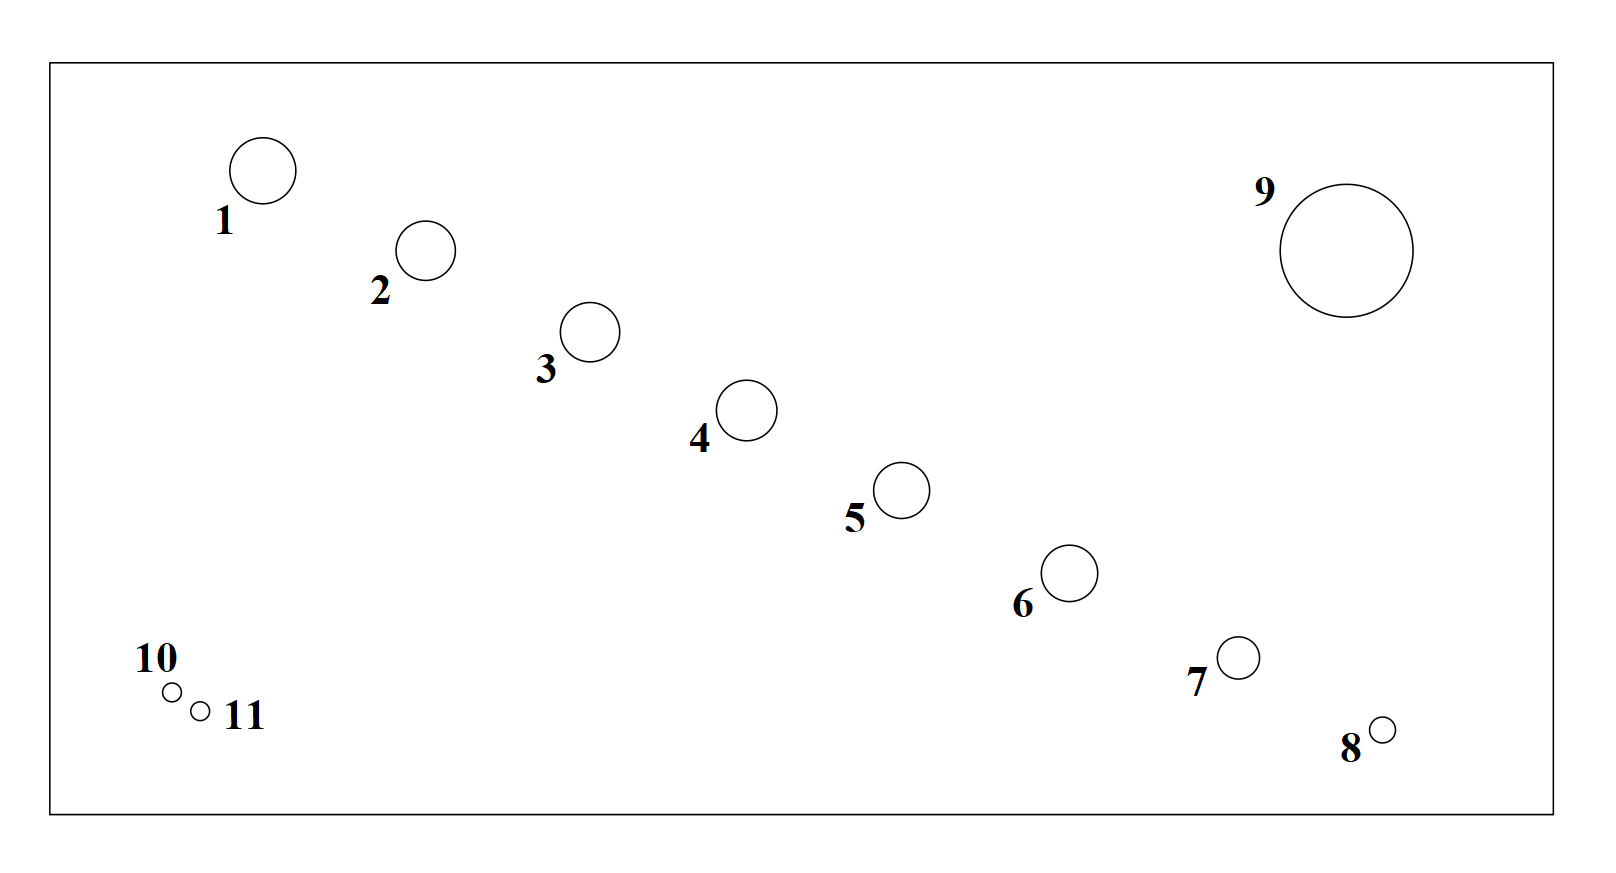
\includegraphics[width=\textwidth]{content/Acrylblock.png}
    \caption{Dies ist eine Skizze des verwendeten Acrylblocks, den Fehlstellen wurden Nummern zugewiesen, auf die im Folgenden referenziert wird. \cite{vUS2}.}
    \label{fig:acrylskizze}
\end{figure}

Zuerst wird mit der händischen Vermessung des Acrylblocks begonnen. Dabei werden sowohl die Gesamtmaße des Blocks, wie auch die einzelnen Positionen und Größen der zu 
untersuchenden Störstellen bestimmt. Nun wird das Ultraschallechoskop in Betrieb genommen und das Programm \textit{A-Scan} gestartet. Der Acrylblock muss mit 
einer ausreichend großen Menge destilliertem Wasser benetzt werden. Mit Hilfe der grafisch dargestellten Peaks werden die Laufzeiten des Signals für sieben Fehlestellen
bestimmt. Hierzu ist es nicht relevant welche Sonde verwendet wird.
Aus diesen Werten kann in \autoref{sec:Auswertung} die Abweichung zur erwarteten Laufzeit und somit die Dicke der Anpassungschicht bestimmt werden. 
 
Im nächsten Teil des Versuches wird die Lage aller Fehlstellen mit dem A-Scan-Verfahren ermittelt,
wobei die $\qty{2}{\mega\hertz}$ Sonde verwendet wird. Auch hier wird das Ultraschallechoskop 
im Impuls-Echo-Verfahren verwendet. Sobald die Signallaufzeiten für alle Fehlstellen notiert sind, wird der Block auch von der gegenüberliegenden Seite untersucht. 
Die Einstellungen und das Messverfahren sind indentisch zu dem vorherigen. Daraus kann die genaue
Position und die Größe der Fehlstellen im Acrylblock bestimmt werden.

In dem Acrylblock befinden sich zwei Störstellen, welche unmittelbar nebeneinander liegen. Anhand dieser soll nun das Auflösungsvermögen der Sonden untersucht werden. Zuerst wird 
ein A-Scan dieser Stelle mittels der $\qty{1}{\mega\hertz}$ Sonde angefertigt. Dies wird für die $\qty{2}{\mega\hertz}$ Sonde wiederholt. Die jeweiligen Peaks werden als Graphiken
exportiert.

Zuletzt wird nun ein B-Scan des Acrylblocks angefertigt. Dazu wird die $\qty{2}{\mega\hertz}$ Sonde verwendet. Sobald das Programm für den B-Scan gestartet wird,
muss die Ultraschallsonde langsam, mit konstanter Geschwindigkeit, in einer geraden Linie über den Acrylblock geführt werden. 
Dies wird auf beiden Seiten des Acrylblocks durchgeführt. Der jeweils erstellte B-Scan wird gespeichert.
Mittels der beiden Bilder können die Abmessungen der Störstellen berechnet werden. 

Im letzten Teil des Versuches wird ein Brustmodell untersucht, in welchem sich zwei \glqq Tumore\grqq{} befinden. Das Modell ist in \autoref{fig:brust} abgebildet.
Zu Beginn wird die ungefähre Lage der Tumore ertastet. Im A-Scan-Programm werden die Einstellungen des Ultraschallechoskops optimiert. 
Dabei wird getestet welche Einstellungen und welche Sonde die klaresten Ergebnisse liefern. Es sollte eine Ultraschallgel als Kontaktmittel verwendet werden.
Anschließend wird ein B-Scan durchgeführt. Der Scan findet erneut entlang einer geraden 
Linie statt. Es werden solange Scans angefertigt, bis die Art, Größe und Lage des Tumors bestimmt werden kann.

\begin{figure}
    \centering
	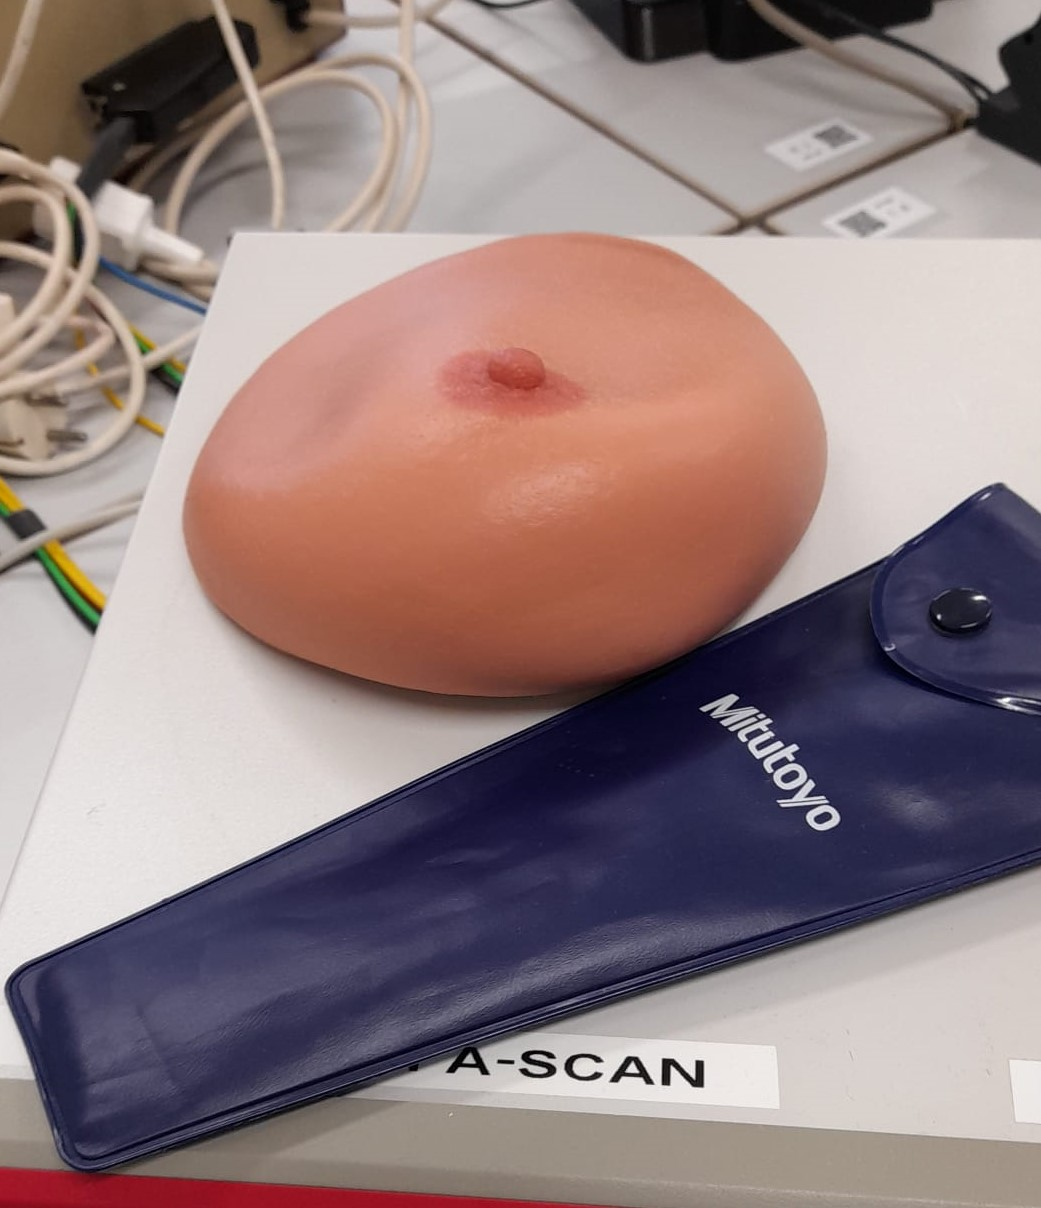
\includegraphics[width=0.5\textwidth]{content/Titte1.jpg}
    \caption{Dies ist ein Bild des verwendeten Brustmodells.}
    \label{fig:brust}
\end{figure}
